\documentclass[15pt,a4paper,oneside]{article}
\usepackage[margin=1in,left=1.5in,includefoot]{geometry}
\usepackage{graphicx}
\usepackage{amssymb}
\usepackage[utf8]{inputenc}
\usepackage{fancyhdr}
\pagestyle{fancy}
\fancyhead{}
\fancyfoot{}

\begin{document}
\fancyhead[L]{Analysis on Hartnell Governor to Improve its Speed Range}
\fancyhead[R]{August 16, 2020}
\fancyfoot[R]{ \thepage\ }
	\begin{titlepage}
		\begin{center}
		\line(1,0){300}\\
		[0.25in]
		\huge{\bfseries Analysis on Hartnell Governor to Improve its Speed Range}\\
		[2mm]		
		\line(1,0){200}\\
		\begin{flushright}
		\textsl{\large August 16, 2020}\\
		[10cm]
		\end{flushright}
		
		\end{center}
		\begin{flushright}
		\textsc{\large Shivam Kumar Pandey}\\
		\textsl{\small Third Year student, IIT Bhubaneswar}\\
		[2cm]
		\textsc{\large Dr. P. B. Ramaiah}\\
		\textsl{\small Assistant Professor, IIT Bhubaneswar}\\
		\end{flushright}
	\end{titlepage}
	\pagenumbering{roman}
	\begin{center}
	
	\section*{Acknowledgement}
	\end{center}
	\addcontentsline{toc}{section}{\numberline{}Acknowledgement}	
	This report is only possible because of the continuous guidance and support of my Professor, Dr. Pattabh B. Ramaiah. His teachings, insights, and enthusiasm have been inspiration to keep me motivated, and I believe this is going to help me further. I am also thankful to all the tutorials and papers I went, that definetly helped learning quick. 
	\\[2cm]
	\begin{flushright}
	\textsl{\small Shivam Kumar Pandey}\\
		\textsl{\small August 16, 2020}\\
\end{flushright}	 
	\pagebreak
	\section*{Abstract}
	\addcontentsline{toc}{section}{\numberline{}Abstract}
	Today, the Science and Technology has evolved so much, that more and more complex processes are now turning into much easier and faster in use. The designs are getting modified, so that their efficiency or insensitiveness might increase. Governors are the speed regulating device, which are being used in a mass scale in Industries. It was first invented in the late 18th century by Watt, then it got further modified as Hartnell or Hartung Governors, which we use today.
	
	This paper mainly foccuses on the design modification of Hartnell governor. We had used arbitrary model and ploted it with MATLAB to find its maximum working range, we had also derived the results comparing the outputs of Modified as well as Hartnell Governor using C Program. The results showed first decrement, then increment, and finally decrement in the value of working range for some specific phi.
	
	These results clearly shows that after certain value of c for specific value of phi, we can modify the design of Hartnell Governor, and can get maximum efficiency from it.
	\paragraph*{Keywords}: Hartnell Governor, MATLAB, C, Working Range 
	\pagebreak
	
	\tableofcontents
	\thispagestyle{empty}
	\pagebreak
	\pagenumbering{arabic}
	
	\setcounter{page}{1}
	\section{Introduction}
	Many Mechanical devices had been used so far for various specific functions, but Governors were used as a speed controller or limiter, designed in the late 18th Century. They do so by regulating the mean speed of the engine, when there are variation in the load. Based on their applications, governors are further classified into two types:
	\begin{itemize}
		\item Centrifugal Governors
		\item Inertia Govornors
	\end{itemize}
	\subsection{Centrifugal Governors}
	A governor whose flyweights respond to centrifugal force to regulate the speed. It is of two types Pendulum type and second is Loaded type. Loaded type governors are further divided into Dead weight loaded, and Spring Loaded Governors. 
	
	Hartnell Governor is a type of spring-loaded Centrifugal Governor with two symmetrical bell crank arms pivoted at point O,O to the frame. The frame is attached to the governor spindle and therefore rotates with it. The helical spring then forces the sleeve through its collar, and this force is adjusted by screwing a nut on the sleeve.
	\subsection{Inertia Governors}
	A governor which utilizes suspended masses that respond to speed changes by reason of their inertia. The advantage of Inerta Governors over Centrifigal Governors is that they respond quickly to the effect of a change of load. But this advantage is very small, as it is very difficult to arrange the governor balls in such a way that the angular acceleration and decceleration of this shaft tend to move their position without disturbing the balance of the rotating part. For this reason, Centrifugal Govenors are preffered over the inertia governors.
	\section{Hartnell Governors}
	Thomas Pickering and William Hartnell invented spring loaded governors that could be operated at higher speeds and were smaller than previous governors, and in the late 17th century, they managed to invent Hartnell Governor. The spindle is driven by the output shaft of the prime mover.\\[1cm] 
	\begin{figure}[h]
	\centerline{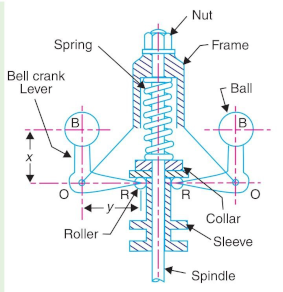
\includegraphics[scale=0.62]{pasted2.png}}
	\caption{Hartnell Governor}
	\label{fig}
	
	\end{figure}\\[1cm]
$$

Let,


m = Mass of each ball in kg

M = Mass of sleeve in kg

r1 = Maximum radius of rotation in mt.

r2 = Minimum radius of rotation in mt.

$\omega1$= Angular speed of the governor at maximum radius in rad/sec

$\omega2$= Angular speed of the governor at minimum radius in rad/sec

S1= spring force exerted on the sleeve at $\omega1$ in N

S2= spring force exerted on the sleeve at $\omega2$ in N

Fc1= Centrifugal force at $\omega1$ in N = m$\omega1^{2}$r1

Fc2= Centrifugal force at $\omega2$ in N = m$\omega2^{2}$r2

k = stiffness of the spring in N/m

x = Length of ball arm

y = Length of sleeve arm

r0 = Distance between O and Governor's axis
$$
h=2\frac{x}{y}\frac{F_{c1}-F_{c2}}{k} = (r1-r2)\frac{y}{x}$
where, F_{c1}=m\omega_{1}^{2}r1 and F_{c2}=m\omega_{2}^{2}r2

and, x, y, and k are constant.
\\[1cm]

Angle between ball arm and sleeve arm is 90 degrees. Now, we consider the same range of motion for comparision (i.e. h1 and h2 are constants) for better analysis of comparision.

\section{Modification in Hartnell Governor Design}
Certain modification are made by mounting the ball slightly below the end of ball arm, and the angle between both the arms is \Phi$ degrees.
\begin{figure}[h]
	\centerline{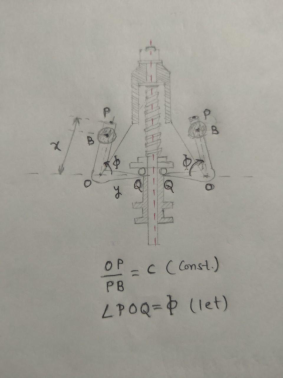
\includegraphics[scale=0.62]{pasted3.png}}
	\caption{Modified design of Hartnell Governor}
	\label{fig}
	
\end{figure}\\[2cm]
\section{Torque Balance Equation}
\begin{figure}[h]
	\centerline{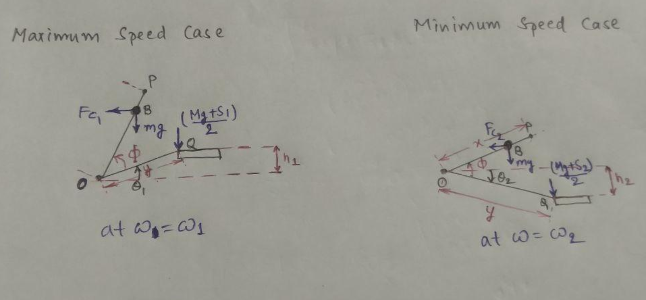
\includegraphics[scale=0.62]{pasted4.png}}
	\caption{FBD of modified design for torque balance}
	\label{fig}
	
\end{figure}\\[2cm]
From fig 2, we see

\begin{equation}
	\frac{OP}{PB}=c
	\label{eq:1}
\end{equation}

So for the Maximum speed case, net Torque about O will be,
\begin{equation}
\label{eq:2}
F_{c1}x\left(\frac{c-1}{c}\right)sin(\theta+\Phi)-mgx\left(\frac{c-1}{c}\right)cos(\theta+\Phi)-y\left(\frac{Mg+S1}{2}\right)cos\theta=0
\end{equation}

considering $cos\theta\rightarrow1$, we get,
\begin{equation}
\label{eq:3}
F_{c1}=mg\left(\frac{\left(cos\Phi-\left(\frac{h1}{y}\right)sin\Phi\right)}{\left(sin\Phi+\left(\frac{h1}{y}\right)cos\Phi\right)}\right)+y\frac{\left(Mg+S1\right)}{2x\left(\frac{c-1}{c}\right)\left(sin\Phi+\left(\frac{h1}{y}\right)cos\Phi\right)}
\end{equation}
Similarly for Minimum speed case, net Torque about O will be,
\begin{equation}
\label{eq:4}
F_{c2}x\left(\frac{c-1}{c}\right)sin(\Phi-\theta)-mgx\left(\frac{c-1}{c}\right)cos(\Phi-\theta)-y\left(\frac{Mg+S1}{2}\right)cos\theta=0
\end{equation}
This Implies,
\begin{equation}
\label{eq:5}
F_{c2}=mg\left(\frac{\left(cos\Phi+\left(\frac{h2}{y}\right)sin\Phi\right)}{\left(sin\Phi-\left(\frac{h2}{y}\right)cos\Phi\right)}\right)+y\frac{\left(Mg+S2\right)}{2x\left(\frac{c-1}{c}\right)\left(sin\Phi-\left(\frac{h2}{y}\right)cos\Phi\right)}
\end{equation}
From fig3,
\begin{equation}
\label{eq:6}
r1=r0-x\left(\frac{c-1}{c}\right)\left(cos\Phi-\left(\frac{h1}{y}\right)sin\Phi\right)
\end{equation}
\begin{equation}
\label{eq:7}
r2=r0-x\left(\frac{c-1}{c}\right)\left(cos\Phi+\left(\frac{h2}{y}\right)sin\Phi\right)
\end{equation}
With these values of r1, r2, $F_{c1}$ and $F_{c2}$, we can finally calculate $\omega_{1}$ and $\omega_{2}$.\\Subtracting [eq:7] from [eq:6], we get,
\begin{equation}
\label{eq:8}
h=h1+h2=\frac{\left(r1-r2\right)y}{x\left(\frac{c-1}{c}\right)sin\Phi}
\end{equation}
Or,\\
\begin{center}
h (Modified Hartnell Governor) = $\frac{c}{(c-1)sin\Phi}$ * h (Hartnell Governor)\\
\end{center}
And, the value of $\frac{c}{(c-1)sin\Phi}>1$ for all cases, because $\frac{c}{c-1}>1$, and $\csc\Phi\geq1$ \\[0.5 cm]This implies,

$sin\Phi\nleqslant$0 (or $180<\Phi<0$) and $c\ne1$
\section{Oservation}
Comparing the expression of height for Hartnell Governor and Modified Hartnell Governor, it is observed that $(F_{c1}-F_{c2})$ is $\frac{\left(c-1\right)sin\Phi}{c}$ times the original one for the same height if mass of balls is ignored. So, if we plot speed vs c graph, for various $\Phi$ values, we get,

Upper speed value is shown with blue line and lower speed value with red line.
\begin{figure}[h]
	\centerline{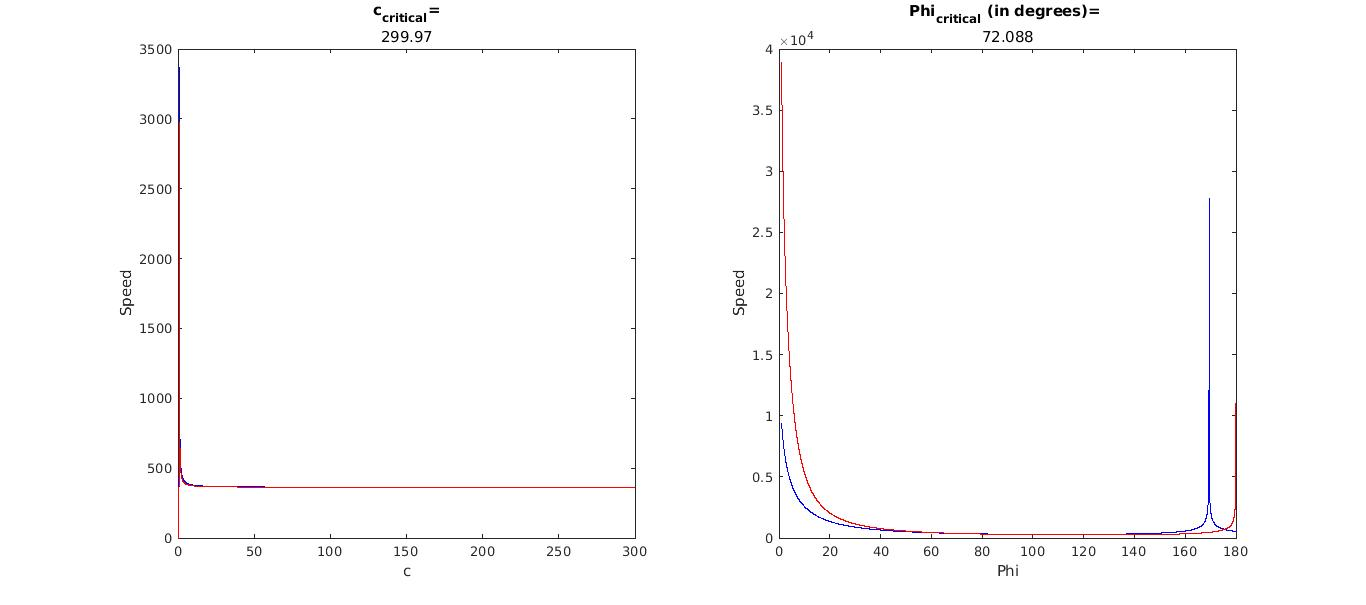
\includegraphics[scale=0.4]{Results.jpg}}
	\caption{(i)For Phi=72.088 degrees, $c_{critical}$=299.97\\(ii) For c=299.97, $Phi_{critical}$=72.088}
	\label{fig}
	
\end{figure}\\[3cm]
This is an zoomed graph to study the initialisation of curve\\
\pagebreak
\\[2cm]
Now for phi= 30, 45, 60 and 90 respectively\\
N vs c plot,
\begin{figure}[h]
	\centerline{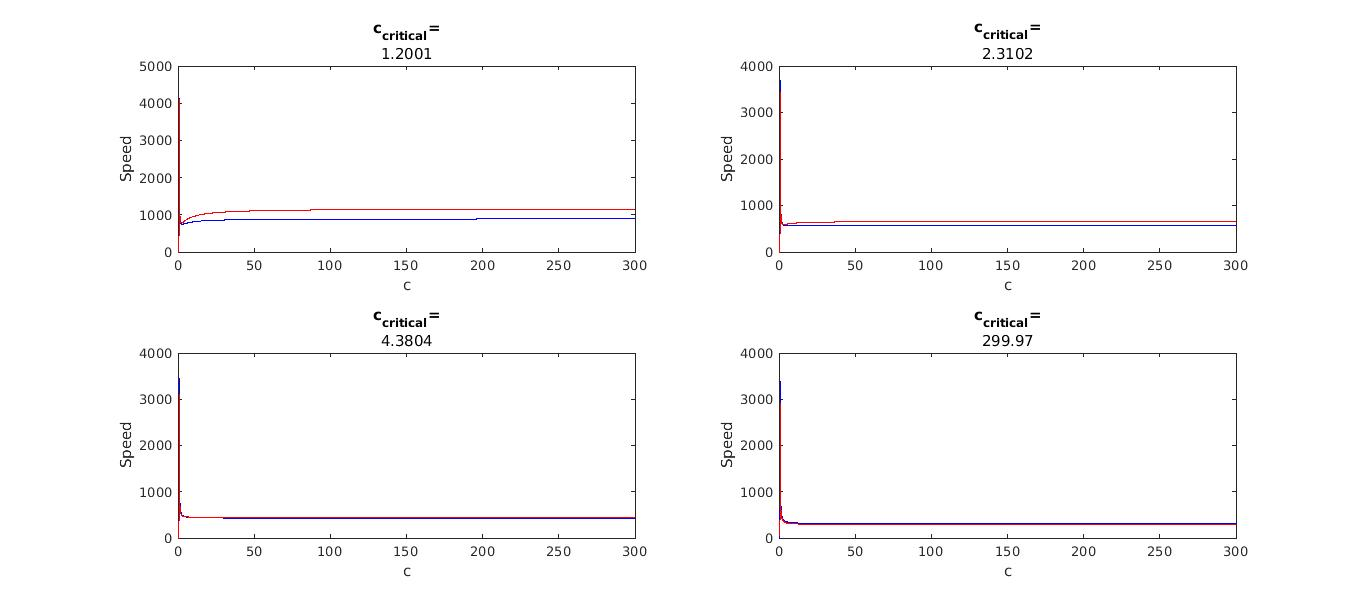
\includegraphics[scale=0.4]{critical.jpg}}
	\caption{(i) For Phi=30 degrees (ii) For Phi=45 degrees (iii) For Phi=60 degrees (iv) For Phi=90 degrees}
	\label{fig}
\end{figure}\\[0.5cm]
Refering to all plot, it seems very clear that for some value of $\Phi$ we are going to get some critical value of c, such that stability of the governor should be maximum at that particular value of $\Phi$. All of the curve seem to converge slowly after some values of c.\\[2cm]
\section{Codes Used}
For comparing the design, I have used C Code:\\
\begin{figure}[p]
	\centerline{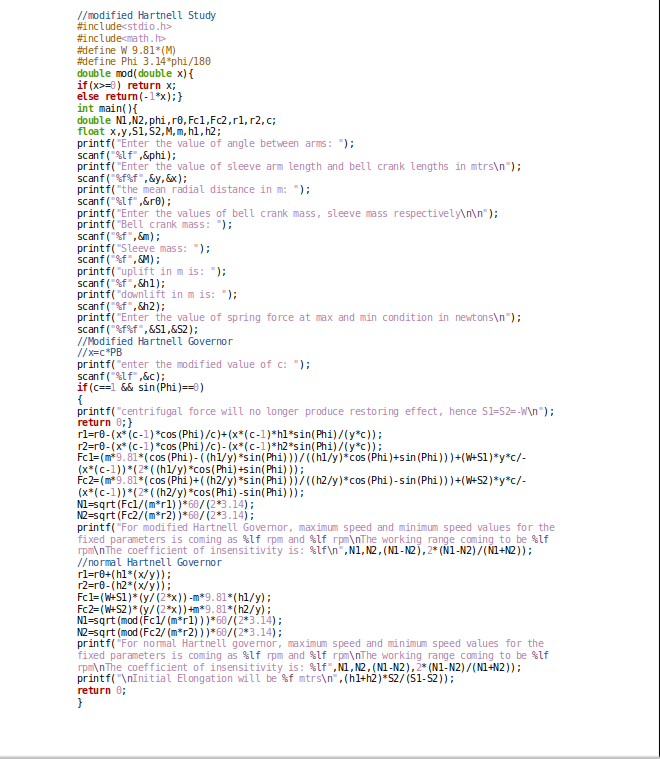
\includegraphics[scale=0.9]{pasted11.png}}
	\caption{C code to compare the results of Modern Hartnell Design with the normal one}
	\label{fig}
\end{figure}\\[10cm]
For Plotting I have used MATLAB:
\begin{verbatim}
clear all;
clc;
\end{verbatim}


\subsection*{Any parametric input can be taken}

\begin{par}
Our Test Case
\end{par} \vspace{1em}
\begin{verbatim}
W=0;
x=0.12;
y=0.08;
m=2.5;
h1=0.015;
h2=0;
S1=1128;
S2=831;
r0=0.12;
\end{verbatim}


\subsection*{Case1: varying c fixing phi}

\begin{verbatim}
c2=linspace(0,300,10000);
Phi2=70; % Can take any arbitrary value
c=c2;
Phi=Phi2;
r1=r0-(x.*(1-(1./c)).*(y.*cosd(Phi)-h1.*sind(Phi))/y);
r2=r0-(x.*(1-(1./c)).*(y.*cosd(Phi)+h2.*sind(Phi))/y);
Fc1=(m*9.81.*(y.*cosd(Phi)-h1.*sind(Phi))./(h1.*cosd(Phi)+y.*sind(Phi)))+((W+S1)*y*y.*c)
./(2*x.*(c-ones(size(c))).*(h1.*cosd(Phi)+y.*sind(Phi)));
Fc2=(m*9.81.*(y.*cosd(Phi)+h2.*sind(Phi))./(-h2.*cosd(Phi)+y.*sind(Phi)))+((W+S2)*y*y.*c)
./(2*x.*(c-ones(size(c))).*(-h2.*cosd(Phi)+y.*sind(Phi)));
N1=sqrt(abs(Fc1./(m*r1)))*60/(2*3.14);
N2=sqrt(abs(Fc2./(m*r2)))*60/(2*3.14);
w=N1-N2;
\end{verbatim}
\subsection*{Search for critical Values}

\begin{verbatim}
for i=1:length(w)
    if w(i)==max(w)
        for j=i:length(w)
            if w(j+1)<0 || j+1==length(w)
                tol=min(w(i:j));
                break;
            end
        end
    end
end
\end{verbatim}
\begin{verbatim}
c_critical=c(find(w==tol));
q=figure;
subplot(1,2,1);
plot(c,N1,'-b');
xlabel('c');
ylabel('Speed');
title('c_{critical}=',num2str(c_critical));
hold on;
plot(c,N2,'-r');
axis auto
hold off;
clear Phi;
clear c;
\end{verbatim}

\subsection*{Case2: varying phi fixing c}

\begin{verbatim}
Phi1=linspace(1,180,10000);
c1=299.97*ones(size(Phi1)); %Can take any arbirary value
c=c1;
Phi=Phi1;
r1=r0-(x.*(1-(1./c)).*(y.*cosd(Phi)-h1.*sind(Phi))/y);
r2=r0-(x.*(1-(1./c)).*(y.*cosd(Phi)+h2.*sind(Phi))/y);
Fc1=(m*9.81.*(y.*cosd(Phi)-h1.*sind(Phi))./(h1.*cosd(Phi)+y.*sind(Phi)))+((W+S1)*y*y.*c)
./(2*x.*(c-ones(size(c))).*(h1.*cosd(Phi)+y.*sind(Phi)));
Fc2=(m*9.81.*(y.*cosd(Phi)+h2.*sind(Phi))./(-h2.*cosd(Phi)+y.*sind(Phi)))+((W+S2)*y*y.*c)
./(2*x.*(c-ones(size(c))).*(-h2.*cosd(Phi)+y.*sind(Phi)));
N1=sqrt(abs(Fc1./(m*r1)))*60/(2*3.14);
N2=sqrt(abs(Fc2./(m*r2)))*60/(2*3.14);
w=N1-N2;
tol=min(abs(w));
index=abs(w)<=tol;
indexNumeric = find(index);
Phi_critical=Phi(indexNumeric(1));
subplot(1,2,2);
plot(Phi,N1,'-b');
xlabel('Phi');
ylabel('Speed');
title('Phi_{critical} (in degrees)= ',num2str(Phi_critical));
hold on;
plot(Phi,N2,'-r');
axis auto;
hold off;
\end{verbatim}\\
\\
\begin{figure}[p]
	Test Case 1:\\
	\centerline{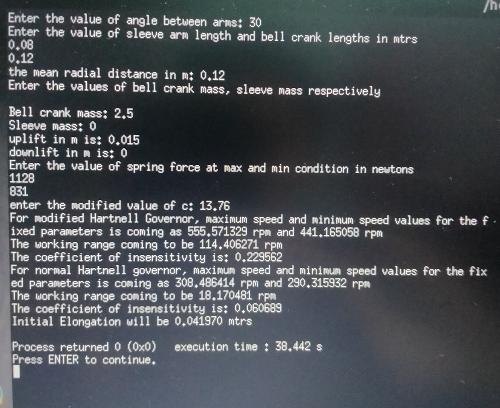
\includegraphics[scale=0.6]{2.png}}
	\caption{Test Case 1}
	\label{fig}
\end{figure}\\
\\[2cm]
\begin{figure}[p]
	Test Case 2:\\
	\centerline{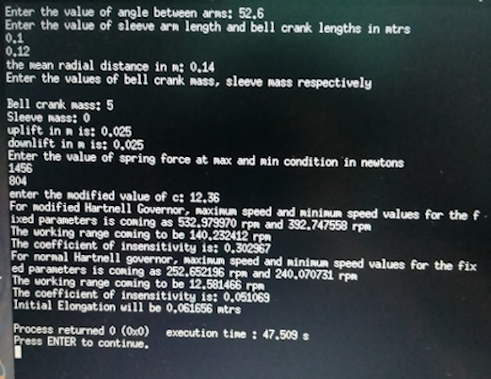
\includegraphics[scale=0.6]{testcase 2 results.png}}
	\caption{Test Case 2}
	\label{fig}
\end{figure}\\
\\[5cm]
\pagebreak
\section{Conclusion}
Hartnell Governor is itself a latest governor which we even use it today. Here in this report, our main concern for modification was to basically increase its working range, and we found out that for certain values of phi and c, we were getting maximum working range which got reduced after sometime. From the test case 1, we found out that for c=13.76, our working range was from 555.57 - 441.16 rpm, while that in case of Hartnell governor was 290 - 308.4 rpm. Also we can find maximum stable Governor through this modification. Thus, it's clear that with this design modification we can enhance the working of a Hartnell Governor.
\section{References}
\bibitem{}Theory Of Machine, fourth edition by S S Rattan

\bibitem{}  International Journal of Scientific and Research Publications, Volume 3, Issue 6, June 2016 | ISSN 2321-2705

\bibitem{} https://in.mathworks.com

\bibitem{} https://nptel.ac.in
\end{document}